% NOTE: must be run with
% xelatex -shell-escape 6_834j_talk
\documentclass[10pt, compress]{beamer}

\usetheme{m}

\usepackage{booktabs}
\usepackage[scale=2]{ccicons}
\usepackage{minted}

\usepgfplotslibrary{dateplot}

\usemintedstyle{trac}

\newcommand{\cmark}{\ding{51}}%
\newcommand{\xmark}{\ding{55}}%

\newcommand{\defeq}{\mathrel{\overset{\makebox[0pt]{\mbox{\normalfont\tiny\sffamily def}}}{=}}}

\title{Robot grocery shopping in partially observable settings}
\subtitle{}
\date{May 13, 2015}
\author{Rodrigo Gomes, Xiaomin Wang, Dustin Tran}
\institute{MIT, 6.834j Cognitive Robotics}

\begin{document}
%(2 min) Background on POMDPs, belief-state MDP, MDP solvers we have
%(2 min) Setup: Grocery shopping as planning in a POMDP
%(4 min) Demo
%(2 min) The solver actually used (value iteration)
%(1 min) Things that failed (Thompson sampling)
%(1 min) Q&A

\maketitle

\begin{frame}[fragile]
  \frametitle{Outline}

  \begin{enumerate}
  \item Background on POMDPs
  \item Grocery shopping as planning in a POMDP
  \item Demo!
  \item What worked
  \item What failed
  \end{enumerate}

\end{frame}

\begin{frame}[fragile]
  \frametitle{Background}

  A \emph{partially observable Markov decision process} (POMDP) is a tuple $(S,A,\Omega,R,T,O)$

  \begin{itemize}
  \item $S$: state space
  \item $A$: action space
  \item $\Omega$: observation space
  \item $R: S \times A \rightarrow \mathbb{R}$ reward function
  \item $T$: transition operator. $T(s' \mid s,a)$ is probability of next state $s'$ given state $s$ and action $a$
  \item $O$: observable operator. $O(o \mid s)$ is probability of observing
  $o$ given at state $s$
  \end{itemize}
\end{frame}

\begin{frame}[fragile]
  \frametitle{Background}

  \begin{figure}[ht]
  \begin{center}
  \centerline{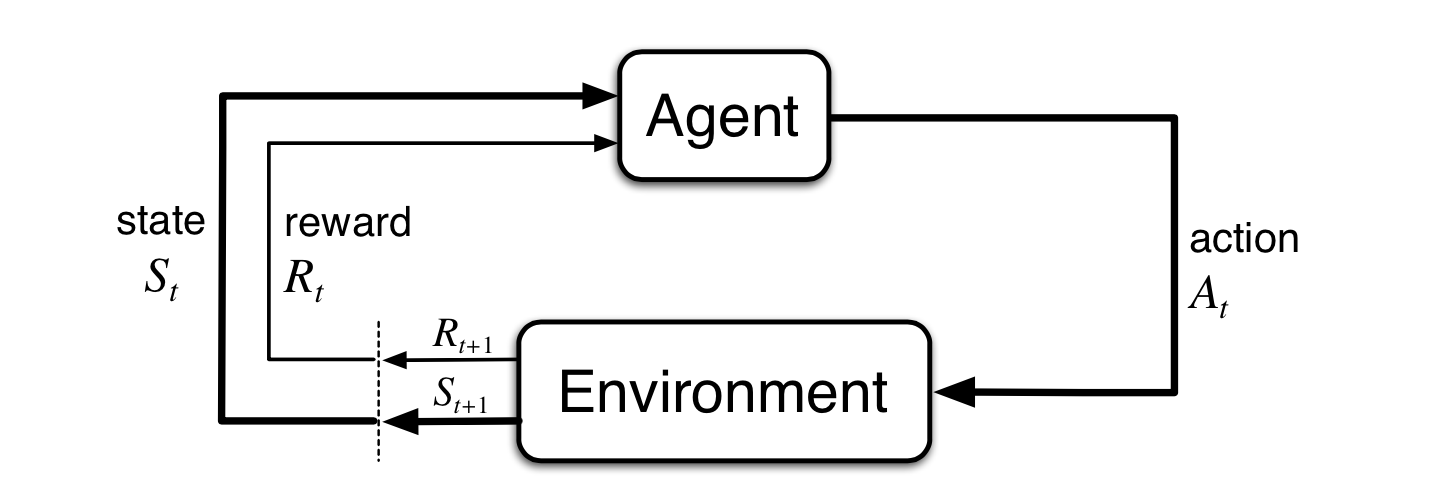
\includegraphics[width=1.25\textwidth]{img/agent_environment_untitled.png}}
  \end{center}
  \end{figure}
\end{frame}

\begin{frame}[fragile]
  \frametitle{Background}
  A POMDP induces an equivalent representation as a \emph{belief MDP} with tuple $(B, A, \tau, R)$

  \begin{itemize}
  \item $B$: set of belief states over the POMDP states
  \item $A$: action space of original POMDP
  \item $\tau$: belief state transition operator\footnote{
  Given $b(s)$, after taking action $a$ and observing $o$ (and reaching state
  $s'$), update belief states
  \begin{equation}
  b'(s') = \frac{P(o\mid b,a,s')}{P(o\mid b,a)}=\frac{O(o\mid s',a)\sum_{s\in S} T(s'\mid
  s,a)b(s)}{\sum_{s'\in S} O(o\mid s',a)\sum_{s\in S}T(s'\mid s,a)b(s)}
  \end{equation}
  }
  \begin{equation*}
  \tau(b, a, b')
  = \sum_{o\in\Omega} P(b'\mid b, a, o)P(o\mid a, b)
  \end{equation*}
  \item $r: B\times A \rightarrow \mathbb{R}$ belief state reward function
  \begin{equation*}
  r(b,a) = \sum_{s\in S}b(s)R(s,a)
  \end{equation*}
  \end{itemize}

\end{frame}

\begin{frame}[fragile]
  \frametitle{Background}
  A POMDP induces an equivalent representation as a \emph{belief MDP} with tuple $(B, A, \tau, R)$

  \begin{itemize}
  \item $B$: set of belief states over the POMDP states
  \item $A$: action space of original POMDP
  \item $\tau$: belief state transition operator\footnote{
  \alert{
  Given $b(s)$, after taking action $a$ and observing $o$ (and reaching state
  $s'$), update belief states
  \begin{equation}
  b'(s') = \frac{P(o\mid b,a,s')}{P(o\mid b,a)}=\frac{O(o\mid s',a)\sum_{s\in S} T(s'\mid
  s,a)b(s)}{\sum_{s'\in S} O(o\mid s',a)\sum_{s\in S}T(s'\mid s,a)b(s)}
  \end{equation}
  }}
  \begin{equation*}
  \tau(b, a, b')
  = \sum_{o\in\Omega} P(b'\mid b, a, o)P(o\mid a, b)
  \end{equation*}
  \item $r: B\times A \rightarrow \mathbb{R}$ belief state reward function
  \begin{equation*}
  r(b,a) = \sum_{s\in S}b(s)R(s,a)
  \end{equation*}
  \end{itemize}

\end{frame}

\begin{frame}[fragile]
  \frametitle{Background}

  Implemented MDP solvers:
  \begin{itemize}
  \item Q-learning
  \item SARSA
  \item R-MAX
  \item Thompson sampling
  \end{itemize}

  There are a lot!
  \begin{itemize}
  \item Function approximations with adaptive basis functions
  \item BOSS
  \item Spectral methods
  \item Skill chaining
  \item $\cdots$
  \end{itemize}

\end{frame}

\begin{frame}[fragile]
  \frametitle{Background}

  Implemented MDP solvers:
  \begin{itemize}
  \item Q-learning \alert{(Watkins, 1989)}
  \item SARSA \alert{(Rummery and Niranjan, 1994)}
  \item R-MAX \alert{(Brafman and Tennenholtz, 2002)}
  \item Thompson sampling \alert{(Strens, 2000)}
  \end{itemize}

  There are a lot more!
  \begin{itemize}
  \item Function approximations with adaptive basis functions \alert{(Mnih et
  al., 2013)}
  \item BOSS \alert{(Asmuth et al., 2009)}
  \item Spectral methods \alert{(Boots et al., 2009)}
  \item Skill chaining \alert{(Konidaris and Barto, 2009)}
  \item $\cdots$
  \end{itemize}

\end{frame}

\begin{frame}[fragile]
  \frametitle{Grocery shopping}

  Setup: Grid World POMDP

  Uncertain movement

  \centerline{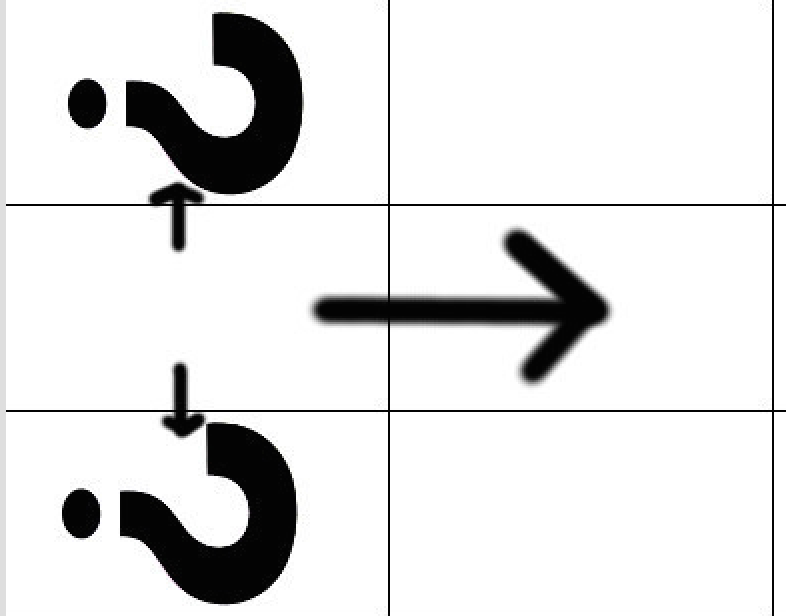
\includegraphics[width=0.22\textwidth]{img/uncertain_transition.png}}

  Can only see around current cell (partially observable)

  \centerline{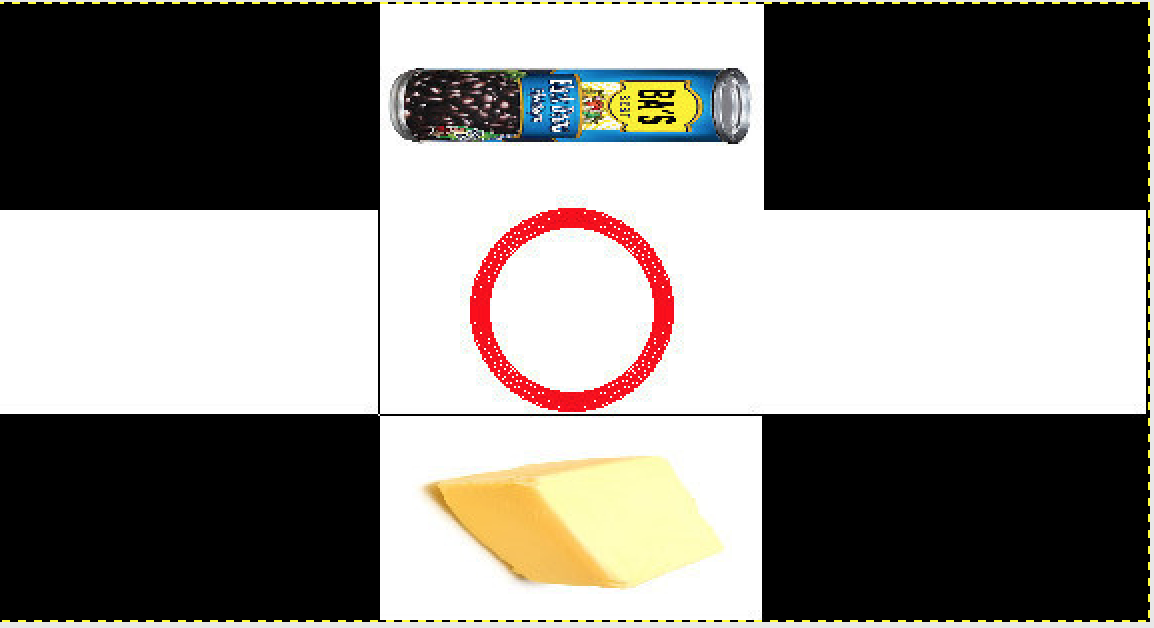
\includegraphics[width=0.22\textwidth]{img/partial_obs.png}}

  World is not fully known beforehand
  \begin{itemize}
  \item Model of how items in the same aisle correlate
  \item Unknown arrangement of aisles
  \item Unknown arrangement of items within aisles
  \end{itemize}
\end{frame}

\begin{frame}[fragile]
  \frametitle{Grocery shopping}

  GUI interface: {\it pygame}

  Every second:
  \begin{itemize}
  \item Agent provides next action based on current belief state
  \item Simulator executes action (errors may happen)
  \item Belief state is updated based on transition probabilities
  \item Belief state is updated based on observation
  \item Belief about the world is updated based on belief state, and observation
  \end{itemize}

  Challenges:
  \begin{itemize}
  \item Markov assumption is not completely accurate
  \item Bias towards increasing probability of most likely states
    % (state increases observation probability, observation increases state probability)
  %\item
  \end{itemize}
\end{frame}

\plain{demo}

\begin{frame}[fragile]
  \frametitle{Our working solver}
  We encode a \textbf{Max Probability} MDP
  \begin{itemize}
  \item Motivated from greedy policies
  \item Choose the most likely state from belief states as one's position in an
  MDP
  \item Solve the MDP!
  \end{itemize}
\end{frame}

\begin{frame}[fragile]
  \frametitle{Our working solver}
  Value iteration:
  \begin{align*}
  v_{k+1}(s) &= \max_a \mathbb{E}[R_{t+1} + \gamma v_k(S_{t+1}) \mid S_t = s, A_t = a] \\
  &= \max_a \sum_{s'} p(s' \mid s,a) [r(s,a,s') + \gamma v_k(s')]
  \end{align*}
\end{frame}

\begin{frame}[fragile]
  \frametitle{Failed tasks}

  \begin{itemize}
  \item Continuous state space in belief MDP: Value iteration
  \item Thompson sampling
  \item TD($\lambda$) methods: Q-Learning, SARSA, Monte Carlo Tree Search
  \end{itemize}
\end{frame}

\begin{frame}
\begin{figure}[ht]
  \frametitle{Most simplified task (GridWorld)}
  \vspace{3ex}
  \begin{center}
  \centerline{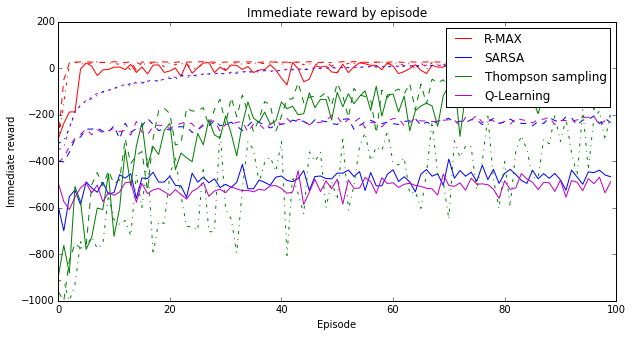
\includegraphics[width=1.1\textwidth]{img/mdp_imm_rewards.png}}
  \end{center}
  \end{figure}
\end{frame}

\plain{
  {\Large Play with it!}\\[5ex]
  
\includegraphics{img/octocat.png}\\[3ex]
  github.com/dustinvtran/bayesrl
}

\end{document}
